\subsubsection{\texttt{RF-8}: automatriculación mediante código de compartición}
\label{subsec:rf8}

Los estudiantes pueden ser matriculados en los cursos manualmente por sus docentes (\referenciaConTT{subsec:rf6}{RF-6}) y, además, tienen la capacidad de inscribirse en cursos por sí mismos utilizando un código proporcionado por sus profesores, ya sea empleando la extensión para Visual Studio Code o a través de la aplicación web. Este requisito es complementario del \referenciaConTT{subsec:rf7}{RF-7}, por el que los docentes disponen de la capacidad para generar códigos de compartición para permitir la autoinscripción de estudiantes en sus cursos.

En caso de querer hacerlo a través de la aplicación web, los estudiantes deben iniciar sesión (\referenciaConTT{subsec:rf1}{RF-1.1}) y, dentro de su página principal, disponen de un campo de texto para introducir el código proporcionado por los docentes, tal como se aprecia en la \referenciaFigura{fig:reqf8-1} y, presionando el botón adyacente, pueden inscribirse en un nuevo curso.

\begin{figure}[ht]
    \centering
    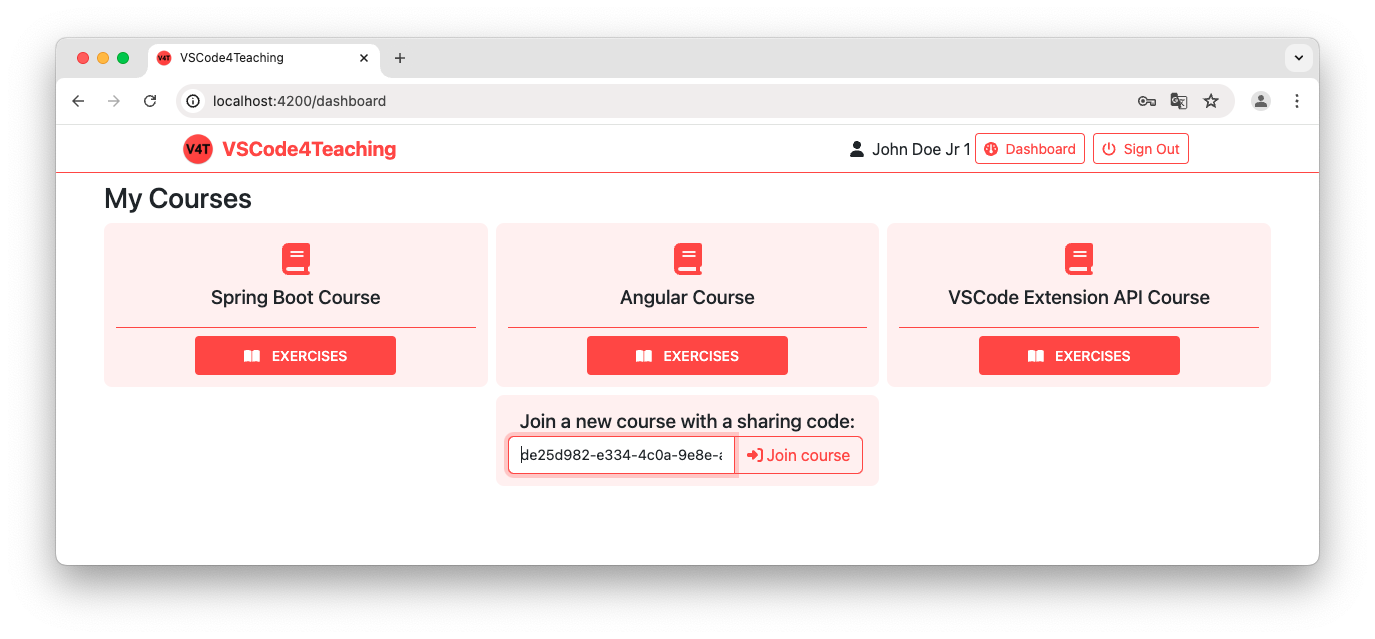
\includegraphics[width=\textwidth]{imagenes/utilizadas/4-3-implementacion/rf8-1.png}
    \caption{Página principal de los estudiantes en la aplicación web con un código de inscripción automática en un curso.}
    \label{fig:reqf8-1}
\end{figure}
